\documentclass[slovene,11pt,a4paper]{article}
\usepackage[margin=1.8cm,bottom=3cm,foot=1.5cm]{geometry}
\usepackage{amsmath}
\usepackage{booktabs}
\usepackage{float}
\usepackage{graphicx}
\usepackage{gensymb}
\usepackage{geometry}
\usepackage{changepage}
\usepackage{subcaption}
\usepackage{multirow}
\usepackage{blindtext}
\usepackage{hyperref}
\usepackage[slovene]{babel}
\pagenumbering{gobble}
\renewcommand{\contentsname}{\centering Contents}

\begin{document}

\title{4. naloga - Populacijski modeli}
\author{Tadej Lozej 28201055}
\maketitle
\begin{center}
Modelska analiza 1 \\
\bigskip
Predavatelj: prof. dr. Simon Širca \\
Asistent: doc. dr. Miha Mihovilovič
\end{center}

\newpage

\tableofcontents

\newpage

\section{Uvod}

\pagenumbering{arabic}

V nalogi se ukvarjamo s populacijskimi modeli. Uporabni so v mnogo različnih situacijah. V nalogi si bomo ogledali tri različne primere v katerih se te modele prakticira. Na začetku si bomo ogledali populacijski model na modelu epidemije. Ogledali si bomo več različnih modelov s katerimi napovedujemo širjenje epidemije. Kot drugi primer populacijskih modelov si bomo ogledali model zajcev in lisic (model Lotka-Volterra) in nazadnje še populacijski model laserja.

\section{Model epidemije}

Kot prvi primer, pri katerem so populacijski modeli uporabni si oglejmo model epidemije. Začeli bomo s preprostim modelom, v katerem populacijo razdelimo v tri razrede, in sicer dovzetne, bolne in imune. Nato si bomo ogledali še primer pri katerem bolne razvrstimo v več stadijev okužbe. Na začetku bodo osebki okuženi, a ne bodo širili epidemije (inkubacijska doba), potem so močno kužni, potem pa v izolaciji in jim kužnost pade.

\subsection{Začetni model}

V začetnem modelu populacijo razdelimo v tri razrede, in sicer dovzetne ($D$), bolne ($B$) in imune ($I$). Dovzetni so zdravi posamezniki, ki jih lahko bolni okužijo, imuni so pa tisti, ki so bolezen uspešno preboleli. V našem modelu bolezen vsi uspešno prebolijo in umrljivosti ni. Populacijski model nastavimo z sistemom diferencialnih enačb

\begin{align}
\dot{D} = -\alpha BD, \\
\dot{B} = \alpha BD - \beta B, \\
\dot{I} = \beta B,
\end{align}
kjer sta $\alpha$ in $\beta$ parametra, ki opisujeta nalezljivost in čas bolezni. Enačbe so s premislekom zelo smiselne. Enačbo (1) razumemo kot, da se dovzetni manjšajo, ko se dovzetni sreča z bolanim, ki okužbo širi. Enačba (2) pravi, da se bolani večajo, ko se bolan sreča z dovzetnim in, da se manjšajo, ko bolan ozdravi. Enačba (3) pa pravi, da se imuni večajo, ko bolani ozdravijo. Vsota dovzetnih, bolnih in imunih je s takšnimi enačbami čez celo epidemijo konstantna, saj če jih seštejemo dobimo na levi odvod vsote na desni pa 0. Rešitev sistema diferencialnih enačb (1)-(3) za vrednosti parametrov $\alpha = 0.8$ in $\beta = 0.2$ in začetnih pogojev
\[D(0) = 0.9, \quad B(0) = 0.1 \quad \text{in} \quad I(0) = 0 \]
prikazuje slika 1. Vidimo potek dovzetnih bolnih in imunih tekom epidemije za model, ki ga predstavljajo enačbe (1)-(3) in omenjene vrednosti parametrov ter začeni pogoji. V našem primeru vidimo, da se ne okužijo vsi dovzetni. Sepravi imamo po koncu epidemije še nekaj ljudi, ki niso imuni. Vidimo tudi, da ima krivulja bolnih očiten vrh. Temu vrhu rečemo vrhunec epidemije in nas v tem modelih še precej zanima, saj se tako lahko ustrezno pripravimo na sprejem bolnikov v bolnicah, sprejemanje ukrepov za preprečanje širjenja itd. Pomembne karakteristike vrha so njegova velikost in čas nastopa. Slika 2 prikazuje te dve karakteristiki vrha epidemije v odvisnosti od parametrov $\alpha$ in $\beta$. Vidimo, da najvišji vrhovi se pojavijo pri veliki nalezljivosti ($\alpha$) in dolgem času bolezni ($\beta$). Velikost teh vrhov sega tudi vse do $63\%$ populacije. Ena očitna lastnost, ki jo lahko razberemo iz slike 2 je ta, da se vrh sploh ne pojavi (oz. pri $t=0\,$s), če $\beta \geq \alpha$. Vidimo, da se v splošnem vrh epidemije pojavi prej za višje vrednosti $\beta$. Enako pa nemoremo reči za vrednosti $\alpha$, saj je to ali vrh nastopi prej ali kasneje, saj izgleda kot, da je to odvisno tudi od parametra $\beta$.

Za ogled več različnih scenarijev epidemije te vrste z različnimi začetnimi pogoji in vrednostmi $\alpha$ in $\beta$ sem pripravil kratko jupiter notebook skripto, ki nam z drsniki omogoča spreminjanje teh vrednosti.

\newpage

\begin{figure}[h!]
\centering
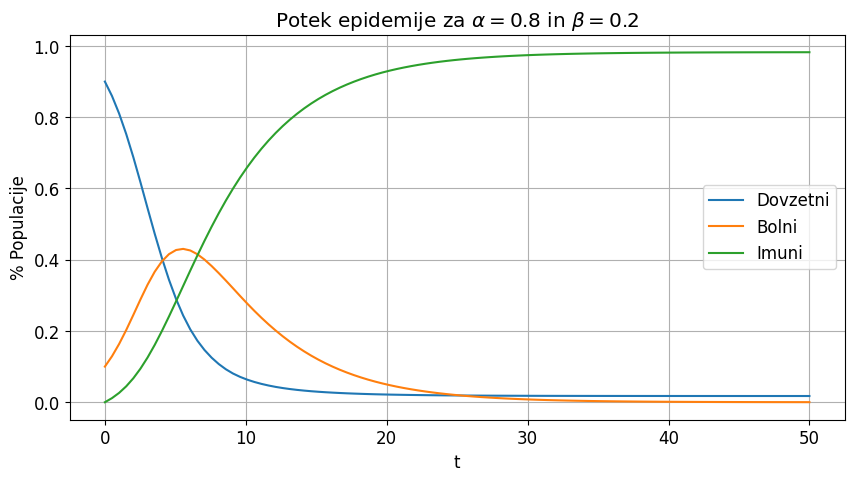
\includegraphics[width=13.5cm]{zacetni1.png}
\caption{Potek epidemije, ki ga napoveduje rešitev sistema diferencialnih enačb (1)-(3) za zgoraj omenjene vrednosti $\alpha$ in $\beta$ ter začetne pogoje.}
\end{figure}

\begin{figure}[h!]
\centering
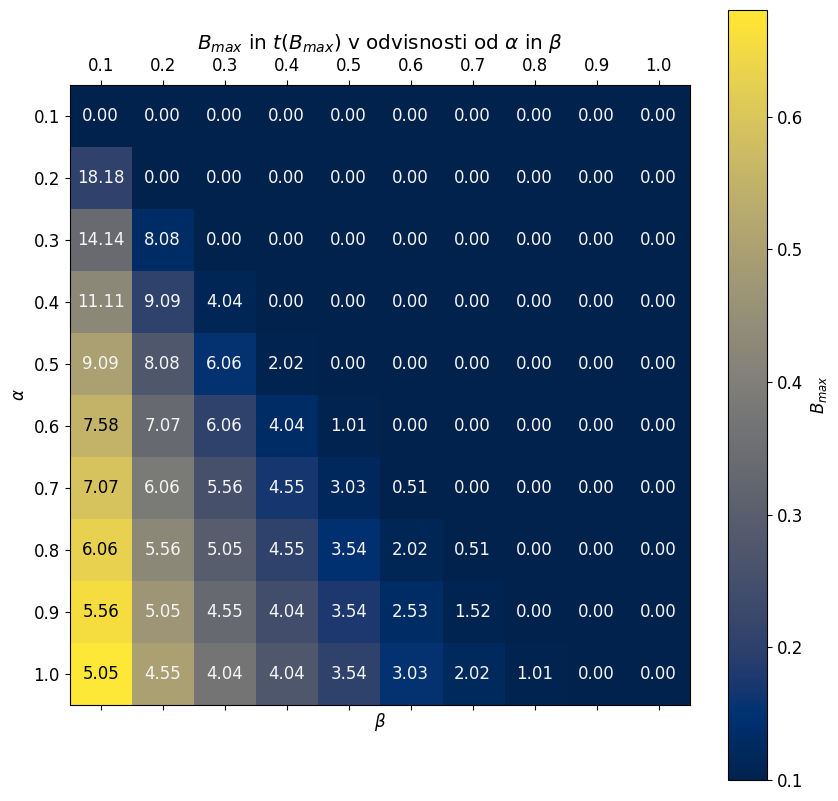
\includegraphics[width=13.5cm]{zacetni2.png}
\caption{Višina in čas nastopa vrha epidemije za različne vrednosti parametrov $\alpha$ in $\beta$. Z barvnim gradientom je prikazana višina vrha, s številko pa čas nastopa vrha epidemije.}
\end{figure}

\newpage

Do zdaj smo se pogovarjali o scenarjih z začetnim pogojem $I(0) = 0$. To pa ni nujno res, saj s cepljenjem lahko zagotovimo začetno imunost in s tem poskušamo omejiti vrh epidemije. Pri parametrih $\alpha = 0.8$ in $\beta = 0.2$ si oglejmo, kako na višino vrha epidemije vpliva začetna imunost populacije. Slika 3 prikazuje višino vrha epidemije $B_{max}$ v odvisnosti od začetne imunosti populacije $I(0)$ za par različnih začetnih vrednosti $B(0)$.

\begin{figure}[h!]
\centering
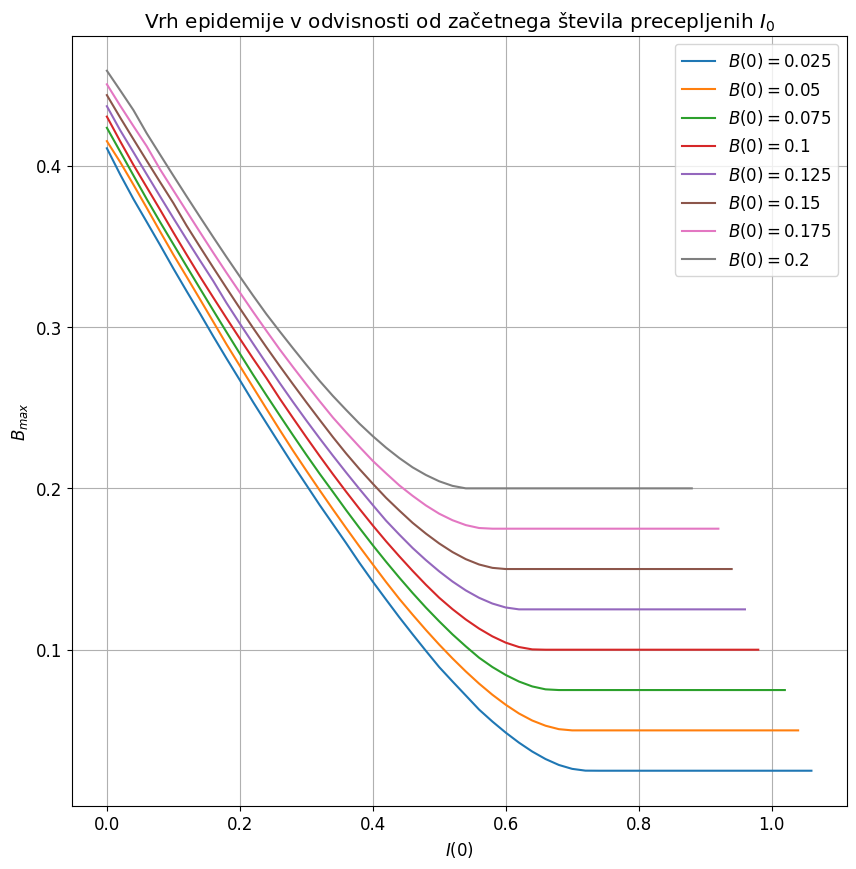
\includegraphics[width=13.5cm]{zacetni3.png}
\caption{Višina vrha epidemije $B_{max}$ v odvisnosti od začetne imunosti populacije $I(0)$ pri vrednosti parametrov $\alpha = 0.8$ in $\beta = 0.2$.}
\end{figure}

Vidimo, da z povečano začetno imunostjo nižamo vrh epidemije. Za vsak $B(0)$ na sliki obstaja tudi takšen $I(0)$, da epidemija vrha sploh ne doseže oz. je ta na začetku in ima seveda kar vrednost $B(0)$. Če predpostavimo, da imajo bolnice kapacitete za recimo $20\%$ populacije in da moramo hospitalizirati vse bolne, bi recimo že pri $B(0) = 0.025$ morala biti začetna imunost populacije približno $25\%$, da bi ob vrhu epidemije v bolnicah zagotovili dovolj postelj. Pri večjih začetnih vrednostih $B(0)$ pa mora biti začetna precepljenost seveda še večja.

\subsection{Model z več stadiji bolezni}

Začetni model iz prvega podpoglavja lahko takoj izboljšamo tako, da bolezni damo več stadijev. Poskusimo lahko s tremi stadiji: najprej so okuženi, a ne širijo epidemije (inkubacijska doba), potem so močno kužni, potem pa so v izolaciji in jim kužnost pade. To je tudi bolj realen potek epidemije, saj tako upoštevamo tudi naravo virusa (inkubacijska doba) in ljudi (izolacija). Bolne tako razdelimo na tri faze $B_1$, $B_2$ in $B_3$, kjer si te številčno sledijo. Sistem diferencialnih enačb, ki ta model opisuje je

\begin{align}
\dot{D} = -\alpha_1 D B_1 -\alpha_2 D B_2 -\alpha_3 D B_3 \\
\dot{B_1} = \alpha_1 D B_1 + \alpha_2 D B_2 + \alpha_3 D B_3 - \beta_1 B_1 \\
\dot{B_2} = \beta_1 B_1 - \beta_2 B_2 \\
\dot{B_3} = \beta_2 B_2 - \beta_3 B_3 \\
\dot{I} = \beta_3 B_3, 
\end{align}
kjer so $\alpha_i$ in $\beta_i$ parametri za kužnost in čas obolenja $i$-tega stadija bolezni. V našem modelu si izberemo

\[
\alpha_1 = 0.25 \alpha, \quad \alpha_2 = \alpha, \quad \text{in} \quad \alpha_3 = 0.05 \alpha,
\]
kjer je je $\alpha = 0.8$ ter

\[
\beta_1 = 3 \beta, \quad \beta_2 = 3\beta, \quad \text{in} \quad \beta_3 = 3 \beta,
\]
kjer je $\beta = 0.2$. Na ta način imamo spet samo dva parametra $\alpha$ in $\beta$, za katera izberemo enake vrednosti kot v začetnem modelu. Takšna izbera parametrov $\alpha$ nam pove, da smo v prvem stadiju kužni za $75\%$ manj kot v kužnem stadiju in da smo v izolacijskem stadiju kužni $95\%$ manj kot v kužnem stadiju. Takšna izbera parametrov beta pa pravi, da v povprečju trajajo vsi stadiji bolezni enako časa. Skupaj smo pa v povprečju bolani $\beta$ časa, kot v primeru začetnega modela. Za občutek poteka takšne epidemije rešimo sistem diferencialnih enačb, ki ga podajajo enačbe (4)-(8). Na sliki 4 je prikazan potek takšne epidemije za izbrano začetno število okuženih $B_1(0) = 0.1$.

\begin{figure}[h!]
\centering
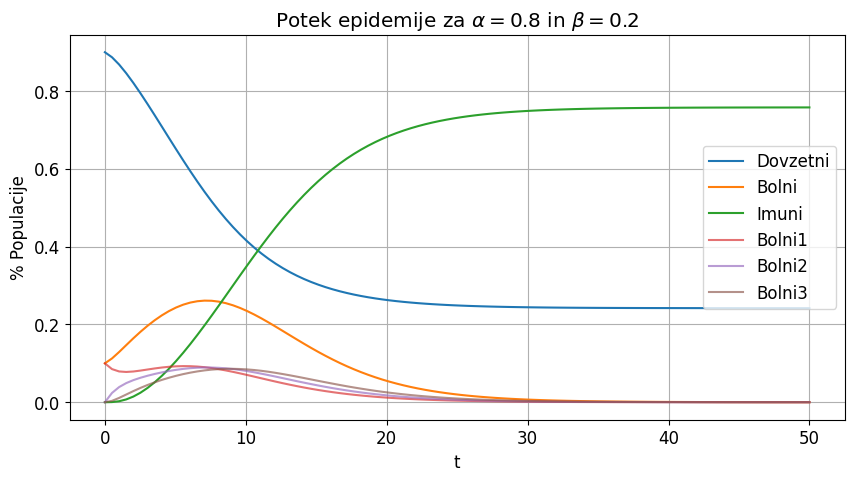
\includegraphics[width=13.5cm]{stadiji1.png}
\caption{Potek epidemije z modelom v katerem bolezen razdelimo v tri stadije. Oranžna črta prikazuje vsoto bolnikov in njen vrh smatramo kot vrh epidemije.}
\end{figure}

Vidimo, da z razmestitvijo bolnikov v stadije v katerih so manj kužni vpliva na vrh in na končno stanje epidemije. Skupno je zbolelo manj populacije kot v začetnem modelu in vrh epidemije je bil manjši. Enako kot v začetnem modelu si oglejmo, kako je višina vrha epidemije in čas njegovega pojava odvisna od parametrov $\alpha$ in $\beta$. Te karakteristike vrhov prikazuje slika 5. Vidimo, da se vrh pojavi tudi nad diagonalo te "matrike". Vidimo, da se z manjšanjem $\alpha$ in večanjem $\beta$ vrh zmanjšuje in pojavlja prej. Razen pri vrednosti $\beta = 0.1$ se z manjšanjem $\alpha$ vrh pojavlja kasneje.

\newpage

\begin{figure}[h!]
\centering
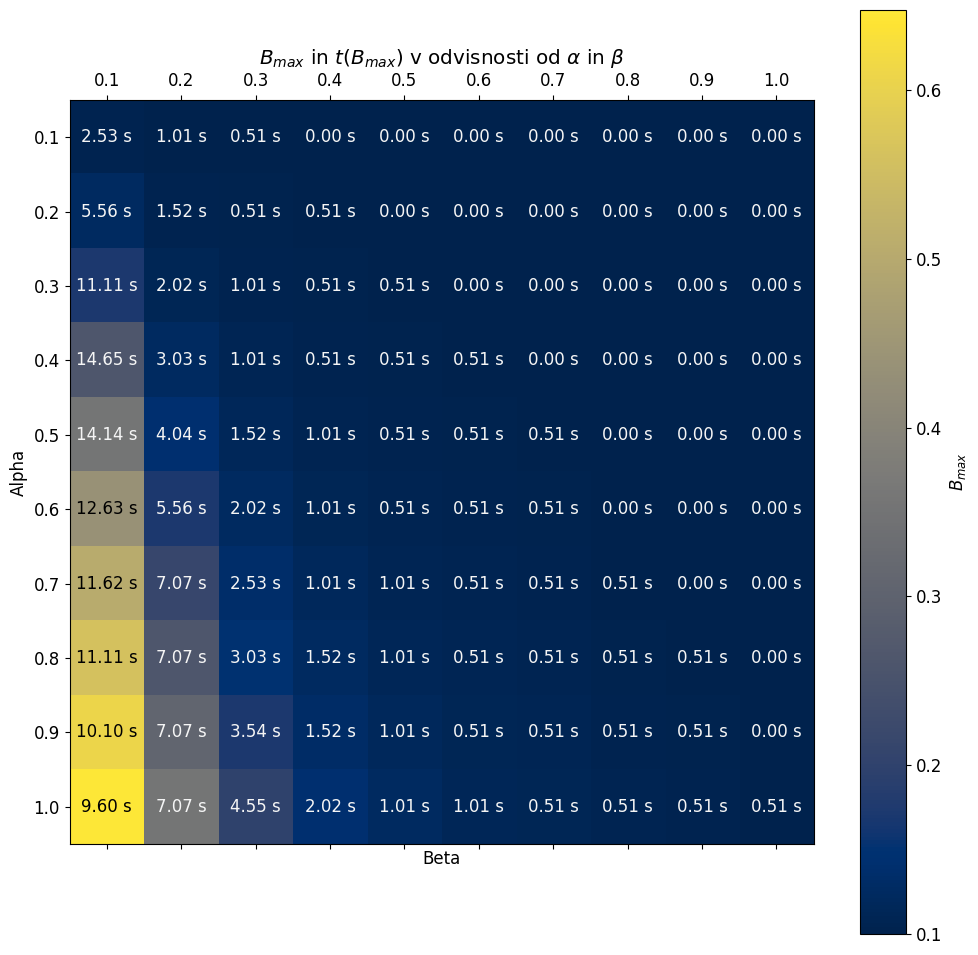
\includegraphics[width=13.5cm]{stadiji2.png}
\caption{Višina in čas nastopa vrha epidemije z modelom v katerem bolezen razdelimo v tri stadije za različne vrednosti parametrov $\alpha$ in $\beta$. Z barvnim gradientom je prikazana višina vrha, s številko pa čas nastopa vrha epidemije.}
\end{figure}

Podobno kot pri začetnem modelu nas tudi tukaj zanima, kako z začetno imunostjo populacije $I(0)$ vplivamo na potek oz. sam vrh epidemije. Na sliki 6 je prikazan graf, ki prikazuje višino vrha epidemije v odvisnosti od začetne precepljenosti pri vrednosti parametrov $\alpha = 0.8$ in $\beta = 0.2$. Vidimo, da so že v splošnem tudi pri ničti začetni imunosti vrhovi v tem modelu manjši kot v začetnem modelu. So pa krivulje veliko bolj položne in kritične precepljenosti so pri večjih $B_1(0)$ večje kot v začetnem modelu.

\newpage

\begin{figure}[h!]
\centering
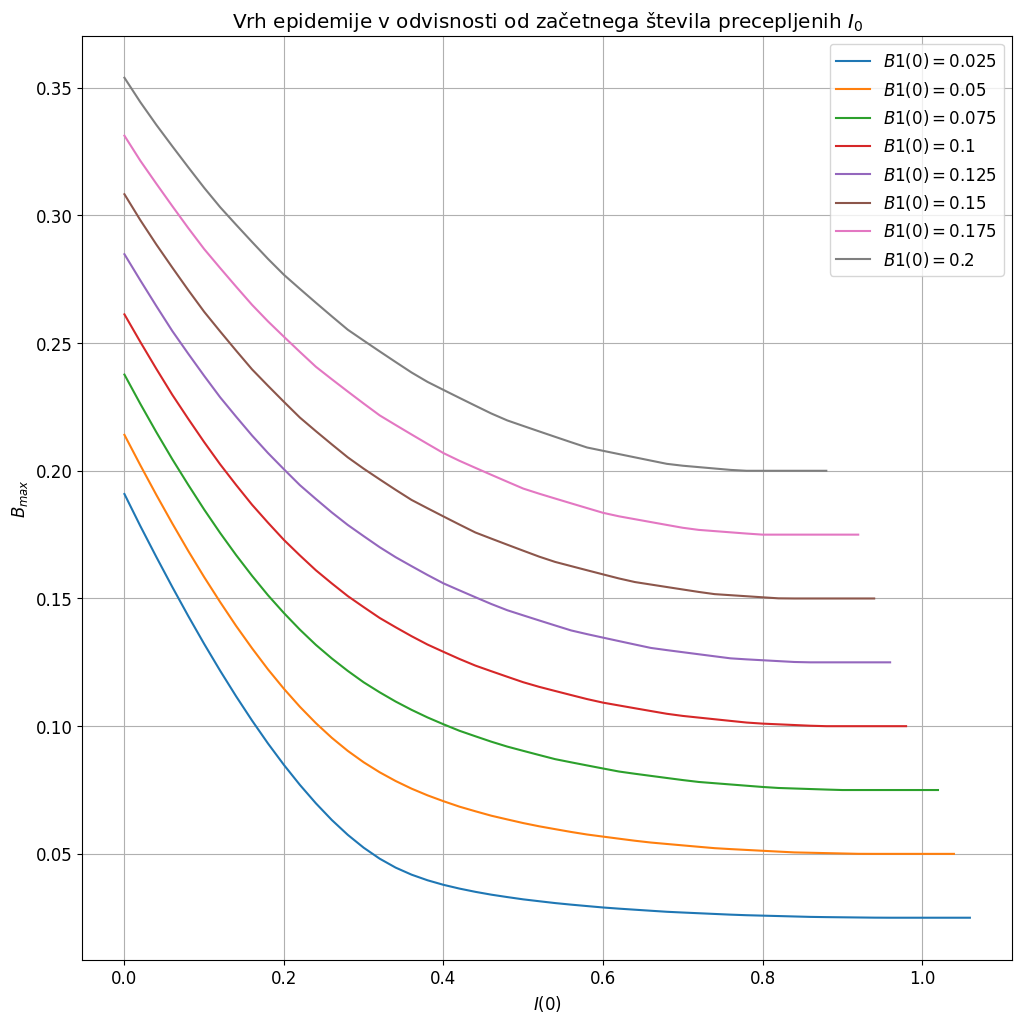
\includegraphics[width=13.5cm]{stadiji3.png}
\caption{Višina vrha epidemije $B_{max}$ pri modelu v katerem bolezen razdelimo v tri stadije v odvisnosti od začetne imunosti populacije $I(0)$ pri vrednosti parametrov $\alpha = 0.8$ in $\beta = 0.2$.}
\end{figure}

\subsection{Primerjava začetnega modela in modela z večimi sadiji}

Primerjajmo, kakšne so razlike v karakteristikah vrhov v odvisnosti od $\alpha$ in $\beta$ med začetnim modelom epidemije in modelu z večimi stadiji. Na sliki 7 je prikazana razlika med višino in časom pojava vrha epidemije med modelom s tremi stadiji in začetnim modelom. Vidimo, da so vsi vrhovi nižji v modelu s tremi stadiji. Za časovni pojav vrha pa v splošnem nemoremo veliko povedati.

Če kritično precepljenost (kritično začetno imunost) definiramo kot začetno vrednost $I(0)$ pri kateri vrh epidemije ne preseže $20\%$ populacije lahko prikažemo kritično precepljenost v odvisnost od začetnega števila obolelih za oba modela epidemij. To prikazuje slika 8. Vidimo, da je kritična precepljenost pri manjših vrednostih $B(0)$ manjša za model s tremi stadiji, za večje vrednosti začetnih obolelih pa se situacija obrne.

\newpage

\begin{figure}[h!]
\centering
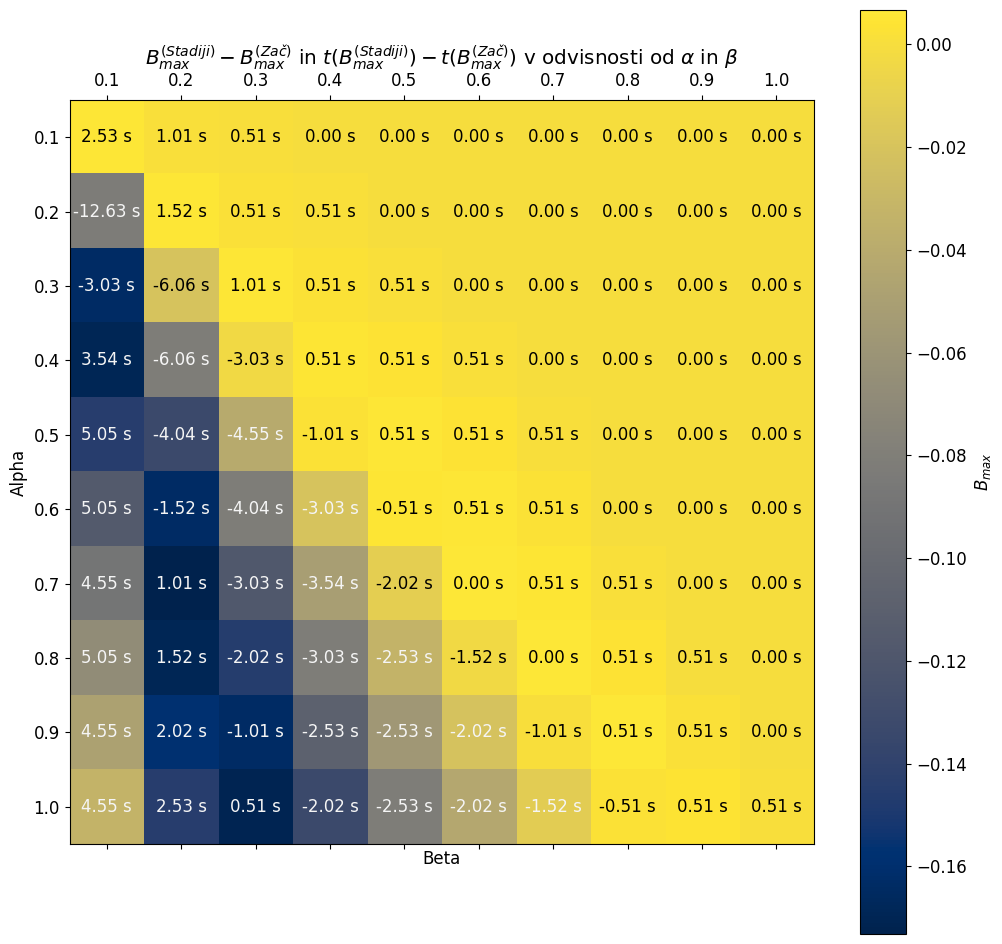
\includegraphics[width=13.5cm]{primerjava1.png}
\caption{Razlika med višino in časom nastopa vrha epidemije med modelom s tremi stadiji in začetnim modelom epidemije za različne vrednosti parametrov $\alpha$ in $\beta$. Z barvnim gradientom je prikazana višina vrha, s številko pa razlika med časom nastopa vrha epidemije.}
\end{figure}

\begin{figure}[h!]
\centering
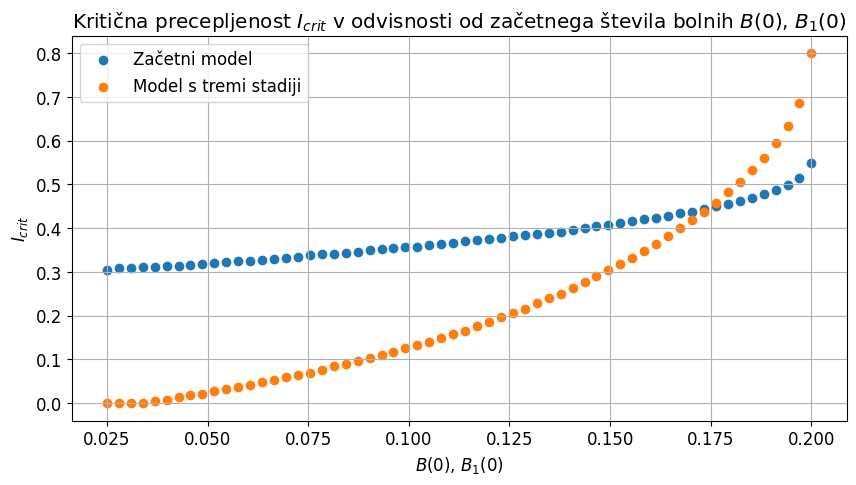
\includegraphics[width=13.5cm]{primerjava2.png}
\caption{Kritična precepljenost v odvisnosti od začetnega števila obolelih za začetni model in model s tremi stadiji pri izbranih parametrih $\alpha = 0.8$ in $\beta = 0.2$.}
\end{figure}

\newpage

\section{Model zajci-lisice}

Preučili bomo standardni deterministični model zajci-lisice (model Lotka-Volterra) v obliki

\begin{align}
\dot{Z} = \alpha - \beta ZL \\
\dot{L} = -\gamma L + \delta ZL,
\end{align}
kjer je $Z$ število zajcev, $L$ število lisic in $\alpha$, $\beta$, $\gamma$ in $\delta$ parametri, ki opisujejo razmnoževanje zajcev, količino pojedenih zajcev, umrljivost lisic in količino dovolj sitih lisic. Problem lahko prevedemo na brezdimenzijski z uvedbo novih parametrov in spremenljivk

\[
l = \frac{\beta}{\alpha} L, \quad z = \frac{\delta}{\gamma} Z, \quad
t = t' \frac{\gamma}{\sqrt{\alpha \gamma}}, \quad p = \sqrt{\frac{\alpha}{\gamma}}.
\]
Tako problem postane enoparametričen. Izbiramo si samo parameter $p$, ki določa koren razmerja med razmnoževanjem zajcev in umrljivostjo lisic. Sistem diferencialnih enačb v brezdimenzijski obliki je

\begin{align}
\dot{z} = pz (1-l) \\
\dot{l} = \frac{l}{p} (l-1).
\end{align}

\subsection{Testiranje metod}

V sistemu zajcev in lisic obstaja invarianta količina, ki se ohranja

\begin{equation}
\delta Z - \gamma \log Z + \beta L - \alpha \log L = konst.,
\end{equation}
kjer je $\log$ naravni logaritem. Problem sem reševal s funkcijo \texttt{scipy.optimize.solve\_ivp}, ki za integratorja lahko uporablja metode \texttt{RK45}, \texttt{RK23}, \texttt{DOP853}, \texttt{Radau}, \texttt{BDF} in \texttt{LSODA}. Ob začetnih pogojih $Z(0) = L(0) = 0.8$ in parametrih $\alpha=\beta=\gamma=\delta=1$ reševal problem od časa $0$ do časa $3000$ in gledal, kako se spreminja teoretična invarianta sistema. Rezultati so prikazani na sliki 9.

\begin{figure}[h!]
\centering
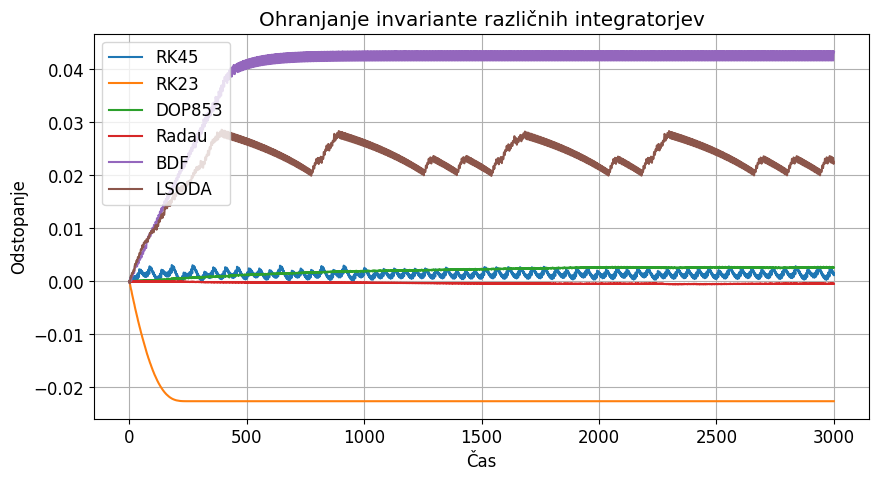
\includegraphics[width=13.5cm]{zajci1.png}
\caption{Primerjava metod v ohranjanju teoretične invariante sistema.}
\end{figure}

Vidimo, da metoda \texttt{BDF} pri izbranih začetnih pogojih najslabše ohranja invarianto sistema, metoda \texttt{Radau} pa jo ohranja najbolje. S to analizo določimo \texttt{Radau} kot našo metodo s katero bomo v nadaljevanju reševali naš problem. V faznem prostoru se ne ohranjanje invariante pozna z odmikanjem od fiksne trajektorije. Na sliki 10 sta prikazani trajektoriji v faznem prostoru za reševanje z integratorjem \texttt{BDF}, ki v tem primeru invarianto slabo ohranja in integratorjem \texttt{Radau}, ki jo v tem primeru dobro ohranja.

\begin{figure}[h!]
\centering
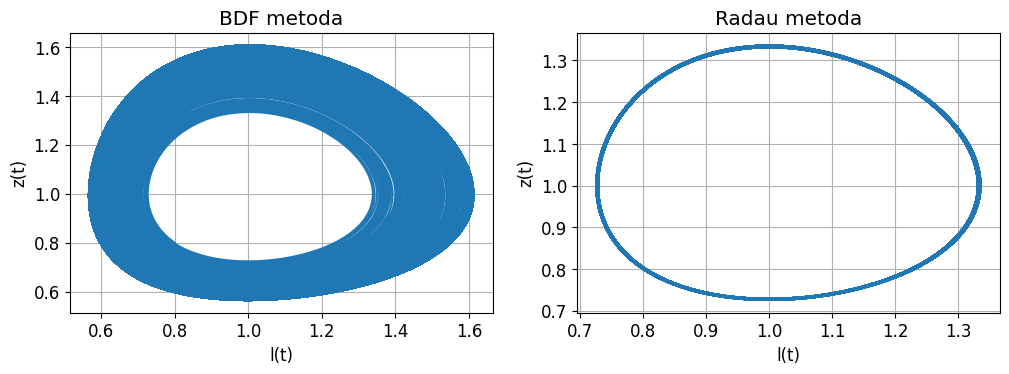
\includegraphics[width=13.5cm]{zajci2.png}
\caption{Fazni prostor zajcev in lisic dobljen z dvemi različnimi integratorji. Na levi z integratorjem \texttt{BDF} in na desni z bolj natančnim integratorjem \texttt{Radau}.}
\end{figure}

\subsection{Fazni diagram}

Rešitev sestema enačb (11)-(12) lahko prikažemo s faznim diagramom $(l(t), z(t))$. Na sliki 11 je prikazan ta fazni diagram pri več možnih začetnih pogojih $z(0)$ in $l(0)$ ter za več vrednosti parametra $p$. Vidimo, da večji kot je parameter $p$ bolj je lik sploščen v $x$ smeri. To pomeni, da ima populacija zajčkov večjo amplitudo nihanja kot lisic. Za manjši $p$ pa velja ravno obratno.

\begin{figure}[h!]
\centering
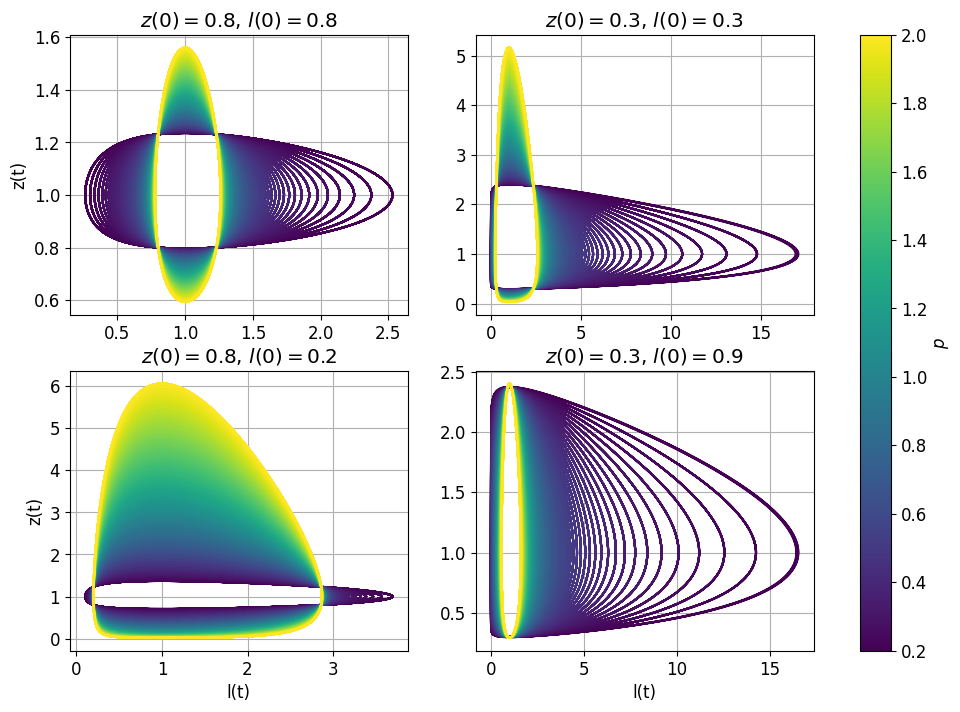
\includegraphics[width=13.5cm]{zajci3.png}
\caption{Fazni diagrami pri različnih začetnih vrednostih $z(0)$ in $l(0)$ ter različnih vrednostih parametra $p$.}
\end{figure}

\subsubsection{Zastojne točke}

Na faznem diagramu je posebej zanimiva okolica fiksnih točk. To so točke, v katerih sta odvoda populacije zajčkov in lisic enaka nič $\dot{z} = \dot{l} = 0$. Iz enačb (11)-(12) lahko razberemo, da na faznem diagamu obstajata dve takšni točki, in sicer točka $(z,l) = (0,0)$ in točka $(z,l) = (1,1)$. Prvo si poglejmo točko $(0,0)$ in obnašanje v njeni okolici.

\begin{itemize}
\item Točka $(0,0)$

Za izračun obnašanja populacij v bližini točke $(0,0)$ lahko v enačbah (11)-(12) nadomestimo vrednosti $z$ in $l$ z 0

\begin{align}
\dot{z} \approx pz \\
\dot{l} \approx - \frac{l}{p}
\end{align}

in enačbi rešimo

\begin{align}
z(t) = z_0 e^{pt} \\
l(t) = l_0 e^{-t/p}.
\end{align}
Vidimo, da gre za eksponentno naraščanje zajčkov, saj ni lisic, ki bi jih jedle, in eksponentno upadanje lisic, saj ni zajcev, ki bi jih jedle. Na sliki 12 je prikazan fazni prostor v bližini točke $(0,0)$ izračunan v omenjenem približku. Pri izračunu je vrednost parametra $p=1$, začetna vrednost populacije lisic pa $l(0) = 0.99$. Začetno vrednost populacije zajcev pa sem spreminjal po $0.0002$.

\begin{figure}[h!]
\centering
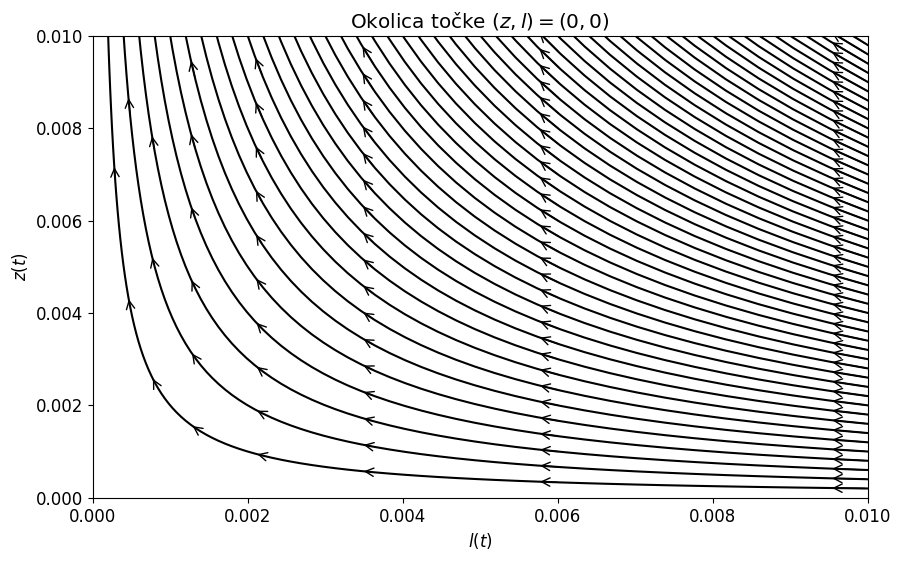
\includegraphics[width=13.5cm]{zajci4.png}
\caption{Fazni diagram v okolici točke $(0,0)$ v približku.}
\end{figure}

\item Točka $(1,1)$

Za izračun obnašanja populacij v bližini točke $(1,1)$ za začetek uvedimo nove spremenljivke $z \rightarrow z+1$ in $l \rightarrow l+1$. Ko nato v enačbah (11)-(12) nadomestimo $z$ in $l$ z vrednostjo $0$ dobimo poenostavljen sistem diferencialnih enačb

\begin{align}
\dot{z} = - pl(z+1) \approx -pl \\
\dot{l} = \frac{1}{p} z(l+1) \approx \frac{z}{p}.
\end{align}
Če eno izmed enačb odvajamo in drugo vstavimo vanjo lahko hitro vidimo, da gre za enačbo nihanja. Podobno kot pri kroženju nabitega delca v magnetnem polju. Slika 13 prikazuje fazni prostor v okolici točke $(1,1)$ po zgoraj navedenem približku. Gre se za odsek elipse oz. nihanja v faznem prostoru. Na sliki je prikazana rešitev ob vrednosti parametra $p=1$ in začetni vrednosti lisic $l(0) = 0.99$. Začetna vrednost zajcev se spreminja od $0.99$ do $1.01$ po koraku $0.0004$.

\begin{figure}[h!]
\centering
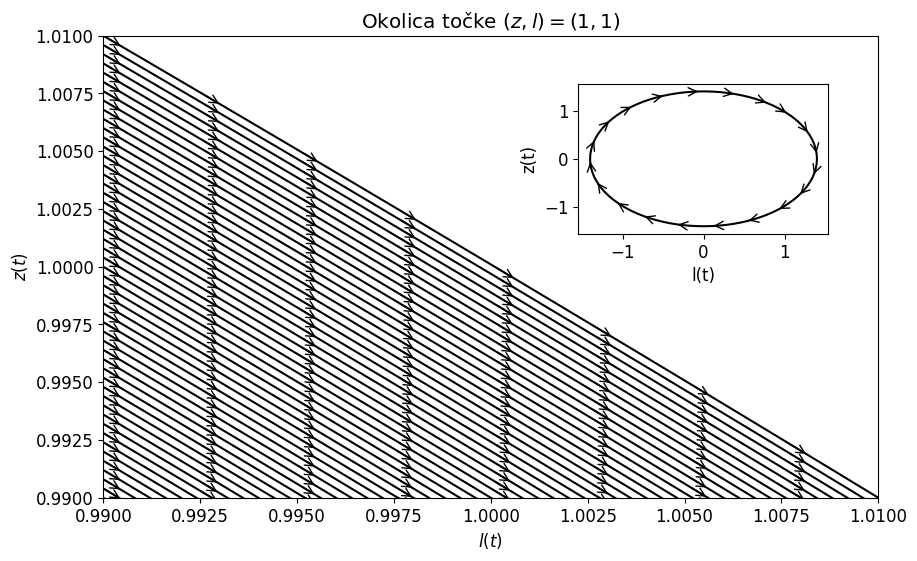
\includegraphics[width=13.5cm]{zajci5.png}
\caption{Fazni diagram v okolici točke $(1,1)$ v približku.}
\end{figure}

\end{itemize}

\section{Populacijski model laserja}

Na zadnje bomo analizirali fazni portret za populacijski model laserja s konstantnim črpanjem.

\begin{align}
\dot{f} = -\alpha f + B af \\
\dot{a} = -\beta a - B af + R,
\end{align}
kjer $f$ predstavlja število fotonov, člena v prvi enačbi predstavljata stimulirano emisijo fotonov in izgube fotonov ter drugi in tretji člen v drugi enačbi spontano sevanje, ki ne koristi produkciji koherentnih fotonov, in kurjavo. Z uvedbo novih spremenljivk

\[
A(t) = \frac{a(t')}{\alpha} B, \quad F(t) = \frac{B}{\beta} f(t') \quad \text{in} \quad t = \sqrt{\alpha \beta} t'
\]
ter novih parametrov
\[
p = \sqrt{\frac{\beta}{\alpha}} \quad \text{in} \quad r = \frac{BR}{\sqrt{\alpha^3 \beta}}
\]
lahko problem prevedemo na brezdimenzijski

\begin{align}
\dot{F} = \frac{F}{p}(A-1) \\
\dot{A} = r - pA(F+1).
\end{align}

\subsection{Fazni diagram}

Na faznem diagramu se nahajata dve zastojni točki, katerih lokacija je odvisna od vrednosti parametov parametrov $p$ in $r$. Na diagramu ju najdemo na mestu $(A,F) = (r/p, 0)$ in $(A,F) = (1, r/p -1)$.

Sistem diferencialnih enačb (22)-(23) rešimo z funkcijo \texttt{scipy.integrate.solve\_ivp}. Rešitve prikažemo posamično v odvisnosti od časa in v faznem portretu na sliki 14. Vrednost parametra $p$ sem izbral $p=0.5$ ter za začetna pogoja vzel $F(0)=A(0)=1$. Rešitve sem nato narisal za več vrednosti $r$ oziroma $r/p$. Na faznem diagramu se lepo vidi konec poteka krivulj v zastojnih točkah. Po tolikšnem času se sistem stabilizira in ostane stacionaren v določeni točki v faznem prostoru. Na sliki 14 vidimo, da s povečevanjem parametra $r$ dosežemo večje populacije fotonov in atomov. Za vrednosti $r$, kjer je $r/p \geq 1$ se laser po nekem času stabilizira v stanju, ki forone oddaja pri menjših vrednostih kvocienta pa ugasne.

\begin{figure}[h!]
\centering
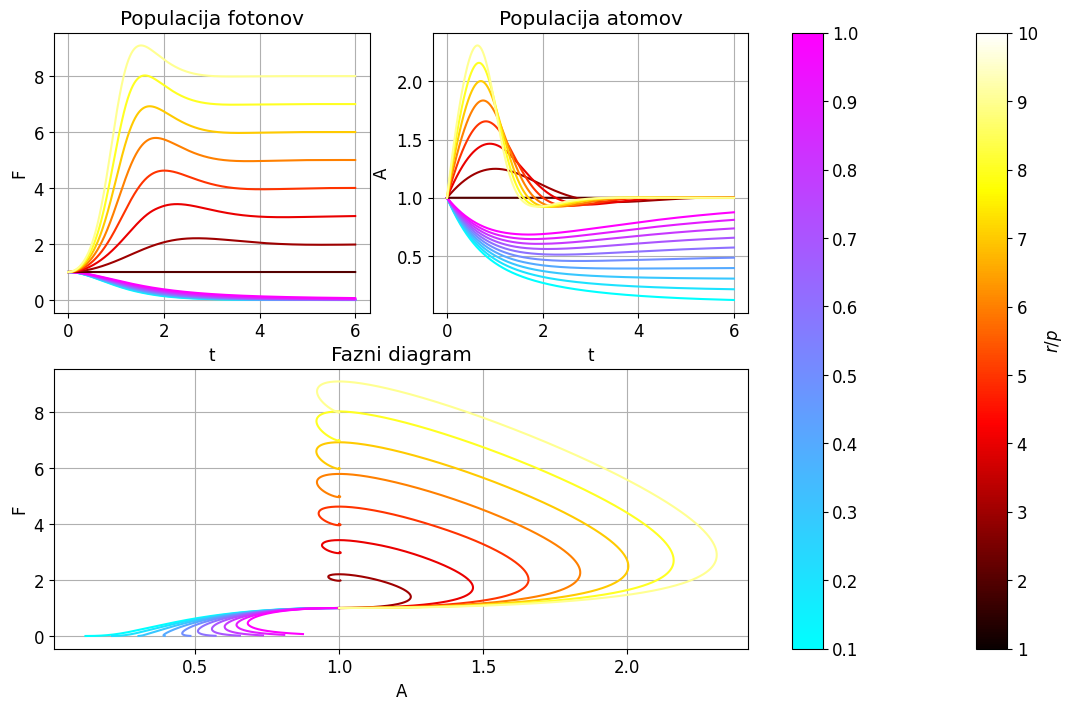
\includegraphics[width=15cm]{laser1.png}
\caption{Populacija fotonov in atomov v odvisnosti od časa ter fazni diagram. Izračunano iz sistema diferencialnih enačb (22)-(23) pri začetnih vrednostih $F(0)=A(0)=1$ ter vrednosti parametra $p=0.5$.}
\end{figure}

Na sliki 15 si lahko ogledamo še fazni diagram pri različnih začetnih pogojih $A(0)$ in $F(0)$. Za izračun sem vzel vrednosti parametrov $p=0.5$ in $r=2.5$. Na grafih se lepo vidi zastojno točko v obeh primerih.

\begin{figure}[h!]
\centering
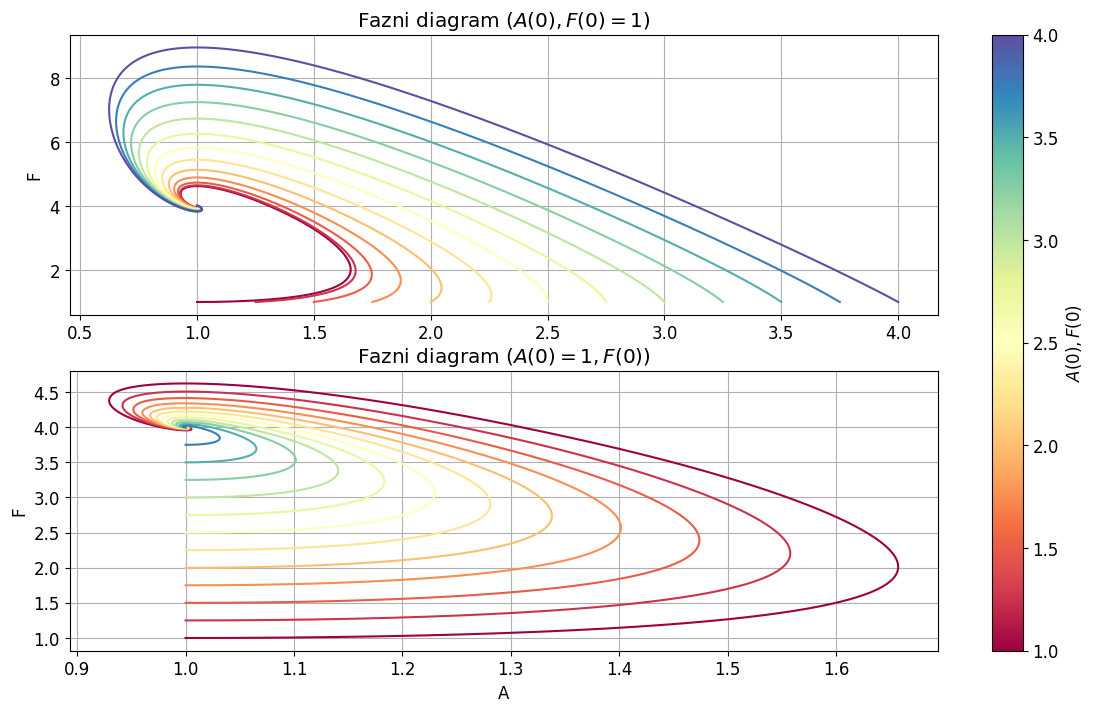
\includegraphics[width=13.5cm]{laser2.png}
\caption{Fazni diagram, izračunan iz sistema diferencialnih enačb (22)-(23) pri vrednostih parametrov $p = 0.5$ in $r = 2.5$.}
\end{figure}

\section{Frekvenca in karakteristični čas oscilacij}

Preden se populacijsko število fotonov ustali na neki vradnosti, le-ta ponavadi prej še nekaj časa niha. Čas in frekvenca nihanja sta odvisni od vrednosi parametrov $p$ in $r$. Na sliki 16 lahko vidimo takšno nihanje. Vidimo, da se v splošnem za večje $r$ laser ustali pri večji končni vrednosti populacije fotonov, kar je obratno za parameter $p$. Prav tako na sliki opazimo, da so z večjim $r$ amplitude nihanja pred ustalitvijo večje in z večjo frekvenco. Obratno pa lahko v tem primeru rečemo za parameter $p$.

\begin{figure}[h!]
\centering
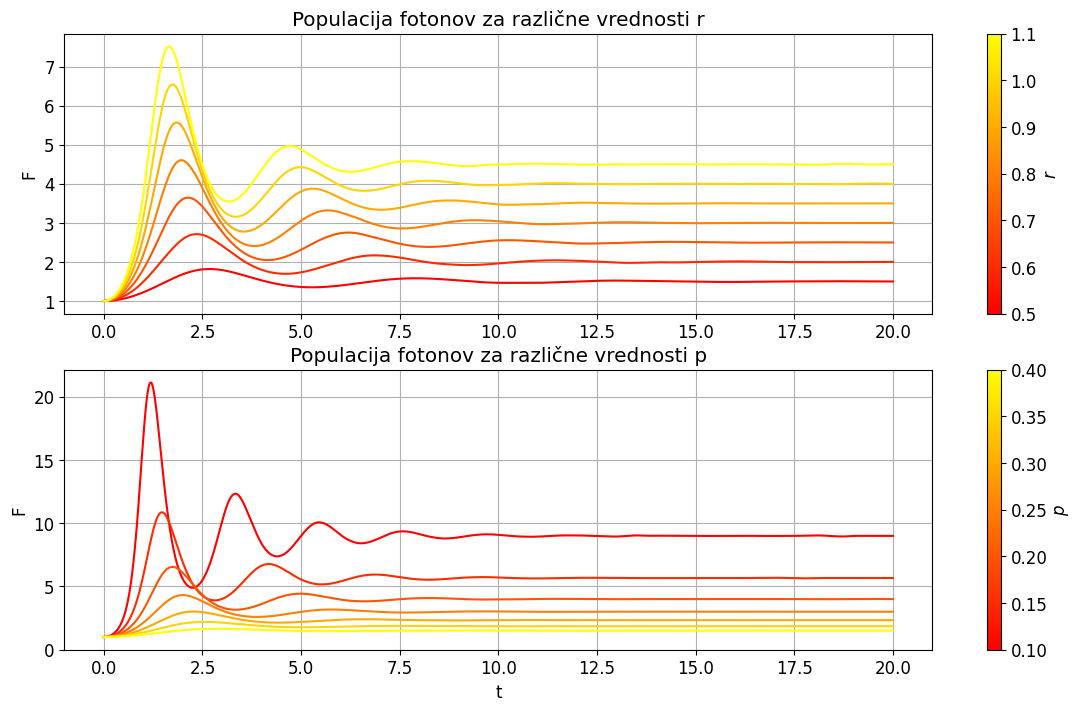
\includegraphics[width=13.5cm]{laser3.png}
\caption{Primer nihanja populacijskega števila fotonov za različne vrednosti $r$ pri $p=0.2$ na prvem grafu in za različne vrednosti $p$ pri $r=1$ a drugem grafu.}
\end{figure}

\section{Zaključek}

Žal mi je za boljšo analizo laserskega populacijskega modela zmanjkalo časa. V mislih sem imel pripraviti še graf, ki bi prikazoval frekvenco in karakteristični čas trajanja nihanja v odvisnosti od parametrov $p$ in $r$. Z analizo drugih modelov sem zadovoljen:)

\end{document}